\documentclass[11pt,]{article}
\usepackage[left=1in,top=1in,right=1in,bottom=1in]{geometry}
\newcommand*{\authorfont}{\fontfamily{phv}\selectfont}
\usepackage[]{mathpazo}


  \usepackage[T1]{fontenc}
  \usepackage[utf8]{inputenc}



\usepackage{abstract}
\renewcommand{\abstractname}{}    % clear the title
\renewcommand{\absnamepos}{empty} % originally center

\renewenvironment{abstract}
 {{%
    \setlength{\leftmargin}{0mm}
    \setlength{\rightmargin}{\leftmargin}%
  }%
  \relax}
 {\endlist}

\makeatletter
\def\@maketitle{%
  \newpage
%  \null
%  \vskip 2em%
%  \begin{center}%
  \let \footnote \thanks
    {\fontsize{18}{20}\selectfont\raggedright  \setlength{\parindent}{0pt} \@title \par}%
}
%\fi
\makeatother




\setcounter{secnumdepth}{3}


\usepackage{graphicx,grffile}
\makeatletter
\def\maxwidth{\ifdim\Gin@nat@width>\linewidth\linewidth\else\Gin@nat@width\fi}
\def\maxheight{\ifdim\Gin@nat@height>\textheight\textheight\else\Gin@nat@height\fi}
\makeatother
% Scale images if necessary, so that they will not overflow the page
% margins by default, and it is still possible to overwrite the defaults
% using explicit options in \includegraphics[width, height, ...]{}
\setkeys{Gin}{width=\maxwidth,height=\maxheight,keepaspectratio}

\title{Mi playa\\
Subtítulo\\
Subtítulo  }



\author{\Large Ana Hilda Valera Arias\vspace{0.05in} \newline\normalsize\emph{Estudiante, Universidad Autónoma de Santo Domingo (UASD)}  }


\date{}

\usepackage{titlesec}

\titleformat*{\section}{\normalsize\bfseries}
\titleformat*{\subsection}{\normalsize\itshape}
\titleformat*{\subsubsection}{\normalsize\itshape}
\titleformat*{\paragraph}{\normalsize\itshape}
\titleformat*{\subparagraph}{\normalsize\itshape}

\titlespacing{\section}
{0pt}{36pt}{0pt}
\titlespacing{\subsection}
{0pt}{36pt}{0pt}
\titlespacing{\subsubsection}
{0pt}{36pt}{0pt}





\newtheorem{hypothesis}{Hypothesis}
\usepackage{setspace}

\makeatletter
\@ifpackageloaded{hyperref}{}{%
\ifxetex
  \PassOptionsToPackage{hyphens}{url}\usepackage[setpagesize=false, % page size defined by xetex
              unicode=false, % unicode breaks when used with xetex
              xetex]{hyperref}
\else
  \PassOptionsToPackage{hyphens}{url}\usepackage[unicode=true]{hyperref}
\fi
}

\@ifpackageloaded{color}{
    \PassOptionsToPackage{usenames,dvipsnames}{color}
}{%
    \usepackage[usenames,dvipsnames]{color}
}
\makeatother
\hypersetup{breaklinks=true,
            bookmarks=true,
            pdfauthor={Ana Hilda Valera Arias (Estudiante, Universidad Autónoma de Santo Domingo (UASD))},
             pdfkeywords = {palabra clave 1, palabra clave 2},  
            pdftitle={Mi playa\\
Subtítulo\\
Subtítulo},
            colorlinks=true,
            citecolor=blue,
            urlcolor=blue,
            linkcolor=magenta,
            pdfborder={0 0 0}}
\urlstyle{same}  % don't use monospace font for urls

% set default figure placement to htbp
\makeatletter
\def\fps@figure{htbp}
\makeatother

\usepackage{pdflscape} \newcommand{\blandscape}{\begin{landscape}}
\newcommand{\elandscape}{\end{landscape}}


% add tightlist ----------
\providecommand{\tightlist}{%
\setlength{\itemsep}{0pt}\setlength{\parskip}{0pt}}

\begin{document}
	
% \pagenumbering{arabic}% resets `page` counter to 1 
%
% \maketitle

{% \usefont{T1}{pnc}{m}{n}
\setlength{\parindent}{0pt}
\thispagestyle{plain}
{\fontsize{18}{20}\selectfont\raggedright 
\maketitle  % title \par  

}

{
   \vskip 13.5pt\relax \normalsize\fontsize{11}{12} 
\textbf{\authorfont Ana Hilda Valera Arias} \hskip 15pt \emph{\small Estudiante, Universidad Autónoma de Santo Domingo (UASD)}   

}

}








\begin{abstract}

    \hbox{\vrule height .2pt width 39.14pc}

    \vskip 8.5pt % \small 

\noindent Mi resumen


\vskip 8.5pt \noindent \emph{Keywords}: palabra clave 1, palabra clave 2 \par

    \hbox{\vrule height .2pt width 39.14pc}



\end{abstract}


\vskip 6.5pt


\noindent  \section{Introducción}\label{introducciuxf3n}

El mar se ha caracterizado como un elemento fundamental al conjunto de
varios factores geologicos y atmosfericos para generar cambios en las
líneas de costas, sean estas en una isla o continente. De acuerdo con
Suárez de Vivero (1999) el termino costa se puede aludir a la franja de
tierra que bordea el mar o a la zona de contacto entre el medio marino y
el medio terrestre. Teniendo en cuenta que la línea de costa puede
variar por un instante o al pasar de los años por la dinámica
morfológica que envuelve esa masa de agua o por causa de fenomenos
naturales que puede traer como posible concecuencia la erosión o
regreción de la costa.

Para Kokot (2004) una erosión costera es el resultado de un exceso de
remoción de sedimentos respecto del aporte suministrado al área en un
determinado periodo. la misma abarca desde la ermersión o sumersión de
sedimentos en las orrillas del mar o la playa, lo que mantiene en
constante movimiento el límite exacto de un verdadero perfil de costa.
Numerosos autores se han dedicado al estudio sobre el análisis de cambio
de perfil de costa teneniendo como referencias imágenes satelitales o
fotografías áereas de años anteriores de la zona de estudio, además de
hacer observaciones y mediciones por un periodo de tiempo determinado
que puedan dar respuesta a dicho cambio o proceso; como es el caso de
(Hernández Santana, Ortiz Pérez, Méndez Linares, \& Gama Campillo,
2008).

La costa como unidad geomorfológica se mantiene en constante estado de
evolución, de ahí la importancia de conocer hacia que lugar se desplaza
más y que forma ésta va adquiriendo, lo que permitirá diferenciar el
tipo de costa existente que de acuerdo con Codignotto (1997) las costas
pueden dividirse en: costa progradación, estacionaria y rotragradación.
De mismo modo el autor hace énfasis de la importancia que és el
comprender los factores que iniciden en este proceso y las causas que la
producen.

La playa de Najayo se encuentra ubicada en la sección que lleva ese
mismo nombre perteneciente al municipio San Gregorio de Nigua provincia
San Cristobal al Sur de la Republica Dominicada en el relieve de la
llanura costera del Caribe bajo las coordenadas geograficas
18º17'40``latitud Norte y 70º06'02''lóngitud Sur;Compone junto a las
provincias Azua, San José de Ocoa y Peravia la subregión de Valdesia. De
acuerdo al mapa geológico de la isla de Santo Domingo se estima que la
formación del relieve costero de Najayo data de la era Cenozoica periodo
Cuaternario entre las época Eoceno-Mioceno, el mismo está compuesto por
arena y gravas bioclasticas formando el cordón litoral, además de
coglomerado, gravas, arenas como fondo de valle y calizas arrecifal,
calciruditas y calcarenitas.

\begin{figure}
\centering
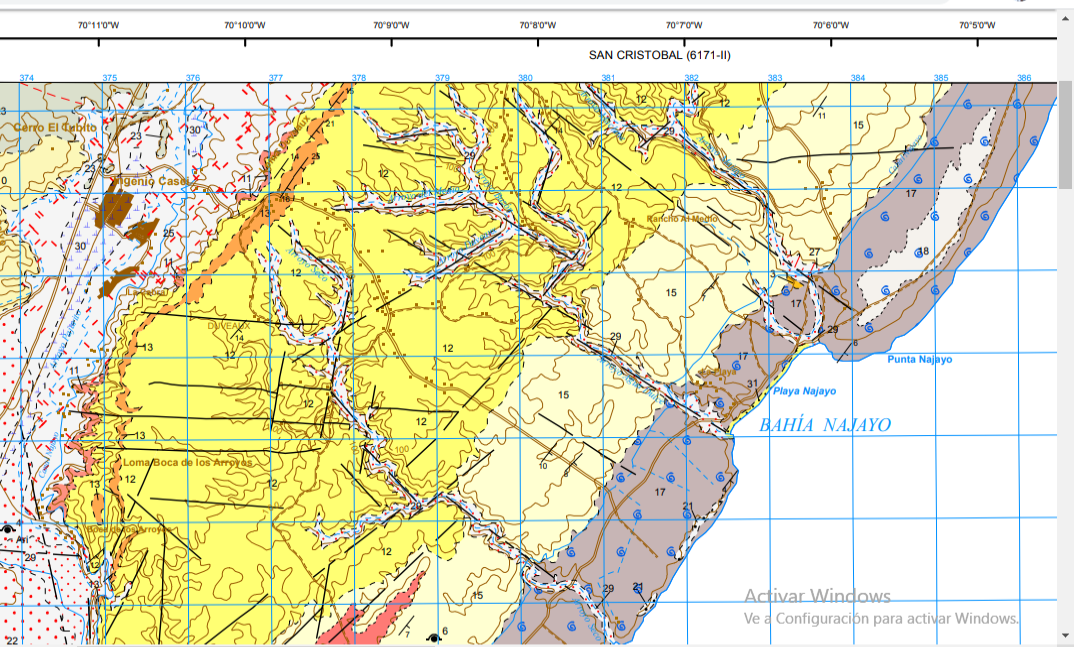
\includegraphics{mapa_bahia_najayo.png}
\caption{mi-manuscrito-anavale}
\end{figure}

\ldots

\section{Metodología}\label{metodologuxeda}

\ldots

\section{Resultados}\label{resultados}

\ldots

\section{Discusión}\label{discusiuxf3n}

\section{Agradecimientos}\label{agradecimientos}

\section{Información de soporte}\label{informaciuxf3n-de-soporte}

\ldots

\section{\texorpdfstring{\emph{Script}
reproducible}{Script reproducible}}\label{script-reproducible}

\ldots

\section*{Referencias}\label{referencias}
\addcontentsline{toc}{section}{Referencias}

\hypertarget{refs}{}
\hypertarget{ref-codignotto1997geomorfologia}{}
Codignotto, J. (1997). \emph{Geomorfología y dinámica costera}.

\hypertarget{ref-hernandez2008morfodinamica}{}
Hernández Santana, J. R., Ortiz Pérez, M. A., Méndez Linares, A. P., \&
Gama Campillo, L. (2008). Morfodinámica de la línea de costa del estado
de tabasco, méxico: Tendencias desde la segunda mitad del siglo xx hasta
el presente. \emph{Investigaciones Geográficas}, (65), 7--21.

\hypertarget{ref-kokot2004erosion}{}
Kokot, R. R. (2004). \emph{Erosión en la costa patagónica por cambio
climático}.

\hypertarget{ref-suarez1999delimitacion}{}
Suárez de Vivero, J. L. (1999). Delimitación y definición del espacio
litoral. \emph{Jornadas Sobre El Litoral de Almería: Caracterización,
Ordenación Y Gestión de Un Espacio Geográfico Celebradas En Almería, 20
a 24 de Mayo de 1997. Pag: 13-23}.




\newpage
\singlespacing 
\end{document}
